\usetikzlibrary{arrows.meta,calc}
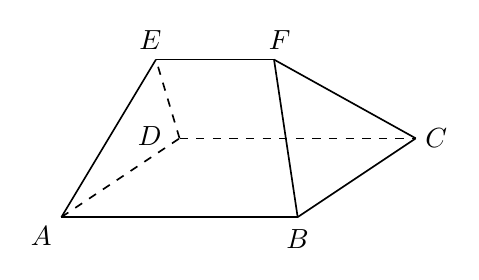
\begin{tikzpicture}[x=1cm,y=1cm,line width=.6pt,font=\normalsize]
\tikzset{ptlabel/.style={font=\normalsize,fill=white,inner sep=1.2pt}}
% Wedge ABCDEF: ABCD square base in oblique view, EF top edge, EF || AB
\coordinate (A) at (0,0);
\coordinate (B) at (3,0);
\coordinate (C) at (4.5,1);
\coordinate (D) at (1.5,1);
\coordinate (E) at (1.2,2);
\coordinate (F) at (2.7,2);
% solid faces
\draw (A) -- (B);
\draw (B) -- (C);
\draw (F) -- (C);
\draw (F) -- (B);
\draw (F) -- (E);
\draw (E) -- (A);
% hidden base edges dashed
\draw[dashed] (A) -- (D);
\draw[dashed] (D) -- (E);
\draw[dashed] (D) -- (C);
% labels offset with white background
\node[ptlabel,below left,xshift=-2pt,yshift=-2pt] at (A) {$A$};
\node[ptlabel,below,yshift=-3pt] at (B) {$B$};
\node[ptlabel,right,xshift=2pt] at (C) {$C$};
\node[ptlabel,left,xshift=-3pt,yshift=1pt,xshift=-2.00bp,yshift=0.00bp,fill=none] at (D) {$D$};
\node[ptlabel,above,xshift=-2pt,yshift=2pt] at (E) {$E$};
\node[ptlabel,above,xshift=2pt,yshift=2pt] at (F) {$F$};
\end{tikzpicture}
